

% **************************** Define Graphics Path **************************
\ifpdf
    \graphicspath{{Chapter6/Figs/Raster/}{Chapter6/Figs/PDF/}{Chapter6/Figs/}}
\else
    \graphicspath{{Chapter6/Figs/Vector/}{Chapter6/Figs/}}
\fi

%*******************************************************************************
\chapter{System Implementation}
\label{ch6}

The experimental evaluations are conducted utilizing the Pepper SR. 
Pepper is a semi-humanoid platform originally developed by Aldebaran Robotics (formerly SoftBank Robotics Europe), engineered specifically for social interaction and affective computing. 
Introduced to the Japanese market in June 2014, the platform remained in production until 2020.

The robot's software architecture provides a suite of Application Programming Interfaces (APIs) for fundamental interaction modalities. 
These encompass speech synthesis and recognition, autonomous navigation, and non-verbal communication, including coordinated gestures and simulated eye contact. 
Figure~\ref{ch6:fig:pepper} depicts the Pepper robot utilized in this study.
%
\begin{figure}
    \centering
    
\includegraphics[width=\linewidth]{Chapter6/Figs/pepper.jpg}
    \caption{Photo of Pepper SR.}
    \label{ch6:fig:pepper}
\end{figure}
%
The version of the Pepper robot utilized in this study is the 1.8 iteration. 
While the hardware specifications remain consistent with previous versions, the development environment utilizes the Android-compatible SDK, enabling the platform to be programmed via Android Studio using Kotlin and Java.

To mitigate the computational limitations inherent in the robot's onboard hardware, a client-server architecture is typically employed. 
In this paradigm, low-level control—including real-time motor actuation and sensor polling—is delegated to the local device, whereas high-level orchestration, such as the Cultural Adapter's inferential logic, is executed on the server side.

In our implementation, the server-side architecture comprises a high-performance laptop workstation running Windows 11. 
The system is powered by an Intel Core i7-13620H CPU, featuring a hybrid architecture of 10 cores and 16 threads with a 24MB L3 cache. 
Memory requirements are supported by 16GB of dual-channel DDR5 RAM operating at a frequency of 5200 MT/s. 
Graphical and parallel processing tasks are delegated to an NVIDIA GeForce RTX 4060 Laptop GPU with 8GB of dedicated GDDR6 VRAM and support for the DirectX 12 API.

\section{Navigation}
\label{ch6:sec:navigation}

Autonomous navigation is defined as the capability of a robotic system to traverse from an initial coordinate (Point A) to a target destination (Point B) without external teleoperation or direct human intervention. 
Within the context of social robotics, this task is further constrained by the requirements of social interaction, most notably the maintenance of appropriate social distance.

This constraint necessitates that the robot adheres to a predetermined spatial radius—derived from proxemic theory—unless environmental obstacles or the proximity of the target goal mandate a dynamic adjustment. 
Various navigation strategies and algorithmic frameworks have been explored in the literature across diverse social settings to optimize this balance between path efficiency and social acceptability.
While various formalizations of social navigation exist within the literature, we developed a specialized solution tailored to the experimental environment, predicated on the following simplifying assumptions:

\begin{itemize}
\item \textbf{Human subjects are treated as static entities:} For the purposes of this study, dynamic human movement was not required. 
While this assumption could be relaxed by implementing real-time human localization and periodic trajectory replanning, such an approach would introduce significant computational complexity beyond the current research scope.
\item \textbf{Spatial Feasibility:} The experimental environment is sufficiently dimensioned to ensure that a feasible path always exists between the robot’s initial pose and the target goal, even when maintaining a maximum comfort distance of 1.5m (representing approximately half of the room's lateral dimension).
\end{itemize}

The Pepper platform natively utilizes a Simultaneous Localization and Mapping (SLAM) algorithm. 
To leverage this capability for server-side high-level control, we generated a static occupancy grid map via the robot’s internal APIs. 
An exemplar of the map produced by Pepper’s mapping suite is illustrated in Figure~\ref{ch6:fig:map}.
\begin{figure}
    \centering
    
\includegraphics[width=0.5\linewidth]{Chapter6/Figs/map_image_1752681775.png}
    \caption{Example of the map generated by Pepper robot.}
    \label{ch6:fig:map}
\end{figure}

Similarly to the mapping process, localization is provided natively via the Pepper APIs. 
However, to mitigate cumulative odometry errors and ensure spatial precision across experimental trials, the robot is manually re-localized prior to the commencement of each session. 

Given these premises, a socially-informed adaptation of the RRT* (Rapidly-exploring Random Tree Star) algorithm was implemented. 
This navigation logic extends the Informed RRT* framework by integrating social constraints directly into the path-planning heuristic.T
he algorithm explores the configuration space until an initial feasible trajectory is identified. 
Upon discovering this first solution, the sampling domain is mathematically constrained to an ellipsoidal subset of the state space, $\mathcal{X}_{sub} \subseteq \mathcal{X}$, defined as:$$\mathcal{X}_{sub} = \{ z \in \mathcal{X} \mid \|z - z_{start}\|_2 + \|z - z_{goal}\|_2 \leq c_{best} \}$$where $c_{best}$ denotes the cost of the current optimal path. 
This restriction focuses the computational resources on improving the existing solution, ensuring asymptotic optimality within the relevant region.
This focused sampling significantly accelerates convergence toward an optimal solution by discarding regions of the configuration space that cannot mathematically yield a more efficient path. 
Concurrently, a rewiring phase continuously optimizes the tree structure by updating parent-child relationships, thereby ensuring asymptotic optimality.

A primary innovation of this implementation is the integration of a human-aware cost function, which explicitly incorporates the social presence and proxemic requirements of the user into the trajectory optimization.
This logic is implemented through a specialized Human class, which extends the base Obstacle class. 
Rather than treating a human as a primitive static collision boundary, the system applies a quadratic penalty to any potential nodes within a specified proxemics radius.
The total cost $C$ of a newly sampled node $z_{new}$ is formulated as:$$C(z_{new}) = C(z_{parent}) + Cost_{dist}(z_{parent}, z_{new}) + \alpha \sum_{h \in H} P(z_{new}, h)$$where $\alpha$ represents a scaling weight and $P(z_{new}, h)$ denotes the proxemic penalty function. 
This penalty is defined piecewise to ensure both hard collision avoidance and soft social compliance:
$$P(node, human) = \begin{cases} \infty & \text{if } dist(node, human) < r_{human} \\ \frac{1}{(dist(node, human) - r_{human})^2} & \text{else if } dist(node, human) < r_{proxemic} \\ 0 & \text{otherwise} \end{cases}$$
The interaction radius $r_{human}$ is not fixed; it is dynamically retrieved from the conversational manager, allowing the robot to adjust its personal space boundaries based on parameters derived from previous empirical experiments. 
By incorporating this penalty, the algorithm inherently prioritizes trajectories that maintain a socially appropriate buffer, steering the planned path away from the user in a manner that preserves human comfort. 
To ensure that the generated path adheres to the kinematic and physical constraints of the Pepper platform, the final sequence of discrete nodes is refined utilizing scipy.interpolate.CubicSpline.
This interpolation step transforms the piecewise-linear path into a continuous, differentiable trajectory $S(t)$, which is significantly more compatible with the robot's drive system and ensures smoother velocity profiles. The resulting spline-based path enables the robot to navigate with high fluidity while strictly adhering to the dynamic social distancing protocols dictated by the real-time interaction state.

%
\begin{figure}
\centering
\begin{subfigure}{0.45\linewidth}
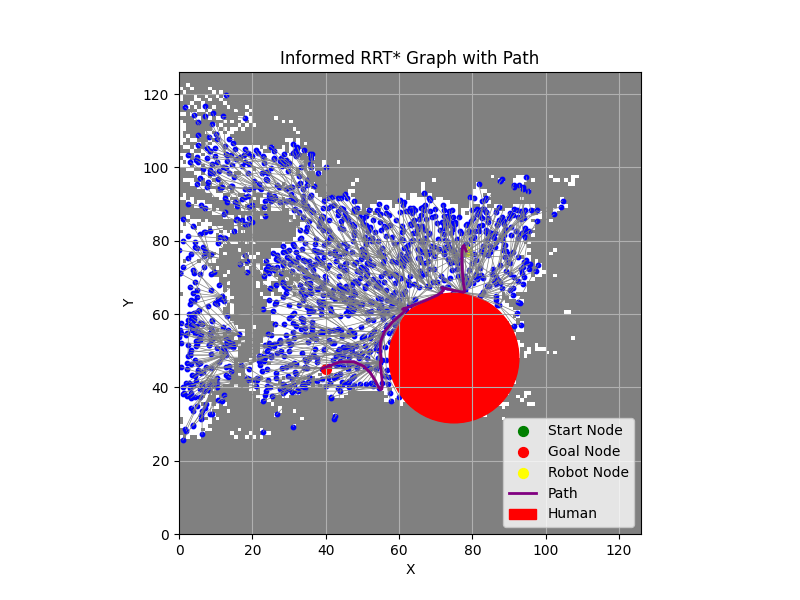
\includegraphics[width=\columnwidth]{Figs/40_45_to_80_80_prox=17.68_back=True.png}
\caption{$r_{human}$=0.893m.}
\end{subfigure}
\begin{subfigure}{0.45\linewidth}
    \centering
    % trim= left bottom right top
    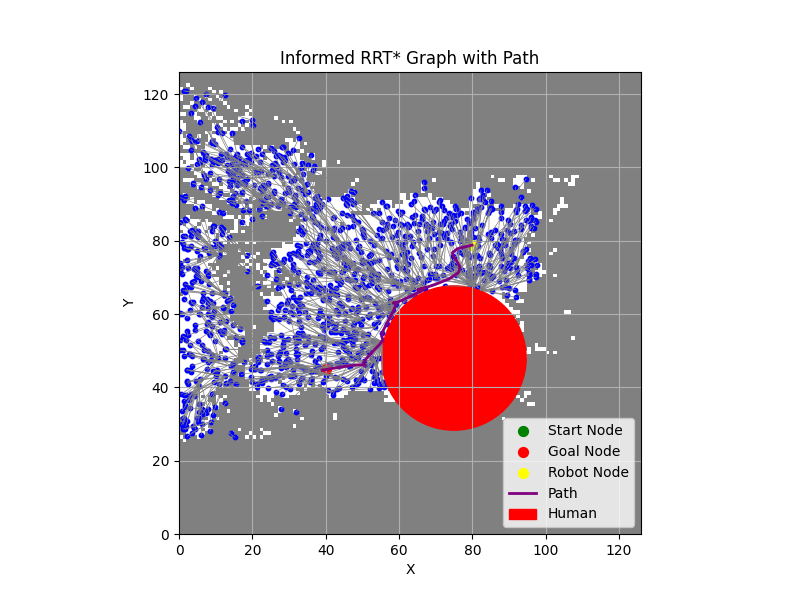
\includegraphics[width=\columnwidth, trim={0 0.4cm 0 0}, clip]{Figs/40_45_to_80_80_prox=19.68_back=True.png}
    \caption{$r_{human}=0.984$m.}
\end{subfigure}
\begin{subfigure}{0.45\linewidth}
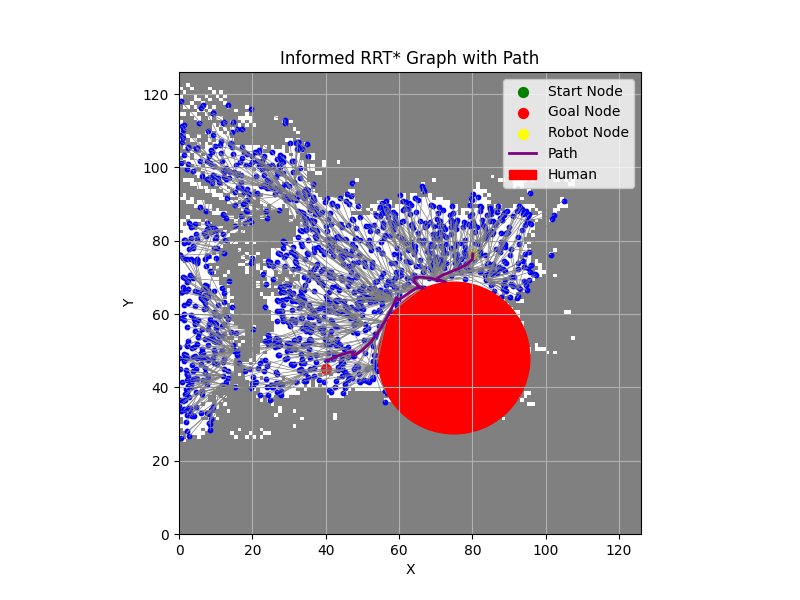
\includegraphics[width=\columnwidth]{Figs/40_45_to_80_80_prox=20.68_back=True.png}
\caption{$r_{human}$=1.034m.}
\end{subfigure}
\begin{subfigure}{0.45\linewidth}
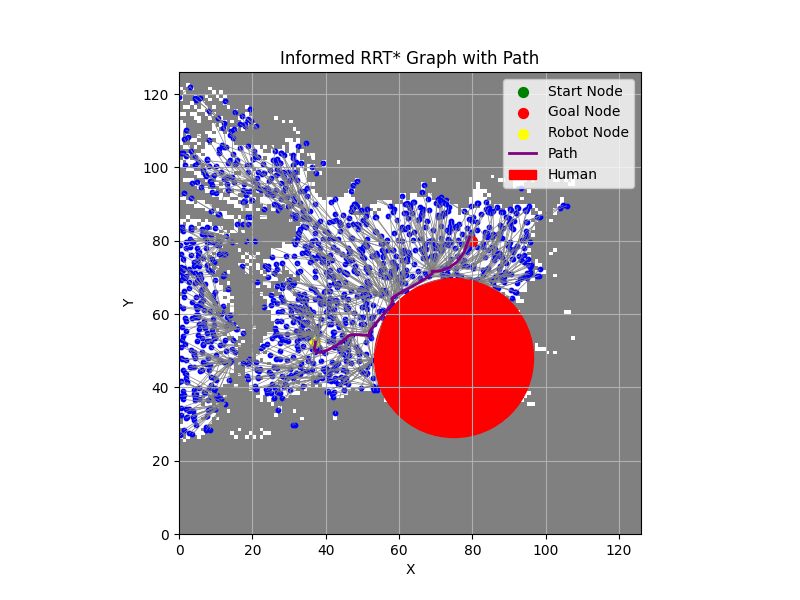
\includegraphics[width=\columnwidth]{Figs/40_45_to_80_80_prox=21.68_back=False.png}
\caption{$r_{human}$=1.084m.}
\end{subfigure}
\caption{Results obtained from robot going from one side to the other side of the room using different values of $r_{human}$.}
\label{ch6:fig:path_res}
\end{figure}
%

Representative results derived from executing this algorithm on the occupancy grid generated by Pepper’s localization suite are illustrated in Figure~\ref{ch6:fig:path_res}.

Upon completing the trajectory generation, the client-side controller receives the optimized path as a discrete sequence of waypoints. 
In the Pepper 1.8 SDK, the GoTo command lacks the continuous path-following capabilities present in earlier iterations; instead, the system must sequentially assign each node as an independent goal. 
The SDK then autonomously generates the motion profile—including acceleration ramps and velocity ceilings—from the current pose to the designated endpoint.

This native implementation would typically result in discontinuous or staccato motion due to repeated deceleration at each waypoint. 
To mitigate this effect, a dynamic filtering strategy was implemented: if the robot is within a predefined proximity threshold of a target node, that node is discarded in favor of the subsequent waypoint. 
This effectively performs a real-time downsampling of the trajectory, allowing the robot to maintain kinetic momentum and ensure smoother transitions between path segments.

\section{Conversation}
\label{ch6:sec:conversation}

The dialogue management system, implemented within the server-side architecture, serves as the cognitive nucleus for the robot's social interactions. 
This module leverages a Llama 3.1 8B LLM to facilitate culturally adaptive communication, enabling the robot to dynamically modulate its linguistic style and content based on inferred cultural parameters.

Each dialogue session is formally structured into four distinct phases: Greetings, Chitchat, Topics, and Goodbye. 
The Greetings phase is managed locally on the client side; upon initialization, the robot delivers a pre-defined utterance, the syntax and tone of which are contingent upon the active experimental paradigm and the user's specific national culture.
%
\begin{table}[]
    \centering
    \begin{tabular}{c|c|c}
       \textbf{Language}  & \textbf{Sentence} \\
         \toprule
        English  & \makecell{Hello, I am Pepper. I will be moving around the room.\\ Talk to me, but please stay where you are.} \\
        \midrule
        German & \makecell{Hallo, ich bin Pepper. Ich bewege mich im Raum.\\ Sprich mit mir, aber bitte bleib, wo du bist.}\\
        \midrule
        Italian  & \makecell{Ciao, sono Pepper. Mi muoverò nella stanza.\\ Parla con me, ma per favore rimani dove sei.}\\
        \bottomrule
    \end{tabular}
    \caption{Greetings sentences.}
    \label{ch6:tab:greetings}
\end{table}
%
These utterances are presented in Table~\ref{ch6:tab:greetings}.

The subsequent dialogue phases are governed by the experimental paradigm, the user's national culture, and specific prompt injection strategies. Transitioning between these states is functionally coupled with the robot's progress along its trajectory. 
Excluding the initial Greetings, the navigational path is partitioned into three segments, with a specific dialogue phase assigned to each spatial interval.

The architecture is structured around three distinct operational paradigms designed to evaluate varying degrees of social intelligence. 
In the Baseline mode, the robot adheres to a set of neutral, non-specialized parameters, utilizing the English language and a low-context communication style paired with a standard interaction distance. 
Conversely, the Foreknowledge mode transitions the system into a proactive state, where culturally specific parameters—including language, communication style, and proxemic preferences—are applied immediately upon the identification of the user.

The most sophisticated configuration of the system is the Adaptation mode, which implements a Natural Language Understanding (NLU) loop to dynamically modulate the robot's persona. Within this paradigm, the system executes secondary LLM inferences to perform a semantic analysis of user inputs, identifying subtle cues regarding preferred communication styles or social distance.

By processing the conversational history, the system can detect if a participant exhibits a preference for indirect, high-context phrasing or a more intimate interaction distance. 
These inferred preferences are utilized to update the robot's internal state in real time, triggering an immediate shift in both the linguistic synthesis and the physical behavior of the Pepper platform via reconfigured proxemic constraints in the navigation stack.

Cultural parameter calibration is rooted in empirical values derived from prior experimental literature, effectively bridging the gap between abstract linguistic styles and physical proxemics. 
The system maintains a repository of cultural profiles, wherein each entity is associated with a specific communication modality and a preferred interaction distance, $D_{pref}$, as established by human-robot interaction (HRI) studies.
For instance, profiles identified as Italian are associated with high-context communication and a distinct $D_{pref}$ value, whereas English and German profiles are mapped to low-context styles with comparatively different spatial requirements. 
When a behavioral shift is detected during the Adaptation phase, these empirically-backed parameters are dynamically injected into the primary LLM's system prompt. 
This architectural alignment ensures that the robot’s synthesized speech—including level of formality and cultural markers—remains synchronized with its spatial positioning, delivering a coherent and socially intuitive user experience.


The \href{https://ollama.com/}{Ollama framework} was utilized as the primary tool for the local deployment of LLMs. The associated Python library enables programmatic orchestration of model weights and inference parameters. For this experimental protocol, Llama 3.1 (\texttt{llama3.1:8b}) was selected. This iteration features 8 billion parameters, a compressed disk footprint of 4.9 GB, and a 128k token context window. Given the architectural estimate of approximately 0.75 words per token, the model supports a functional context of roughly 96,000 words.

Llama 3.1 was chosen specifically for its expansive context window and robust multilingual capabilities\footnote{\href{https://ai.meta.com/blog/meta-llama-3-1/}{https://ai.meta.com/blog/meta-llama-3-1/}}\footnote{\href{https://ollama.com/library/llama3.1}{https://ollama.com/library/llama3.1}}, which are essential for accurately processing the linguistic nuances of the Italian and German languages analyzed in this study.
In the Appendix~\ref{appendix} can be found the complete prompt used for the experiments with its variant for each paradigm.

On the client side, the Pepper platform executes the adaptation by dynamically reconfiguring the Text-to-Speech (TTS) and Speech-to-Recognition (STT) parameters to align with the specific linguistic requirements of each experimental group.

\section{Orchestration and REST API}
The server-side implementation is anchored by a Flask-based REST architecture, which serves as the central orchestration layer for the system's cognitive and navigational functionalities. 
This server acts as a computational bridge between the Pepper robot's Android-based controller and the resource-intensive logic required for path planning and natural language processing.
The architecture is designed to support modular integration, facilitating the simultaneous management of multiple process instances to ensure that the robot's verbal interactions and physical movements remain synchronized and contextually aware. 
A primary responsibility of this layer is the maintenance of the robot's spatial state through real-time data synchronization. 
The system leverages Pepper’s native localization capabilities, asynchronously receiving pose updates—comprising $x$, $y$, and $\theta$ coordinates—via the REST interface.

This integration ensures that the server’s internal representation of the robot node remains consistently aligned with the physical hardware’s odometry and localization filters. 
This state management utilizes a dual-coordinate framework that facilitates seamless transformations between the discrete, pixel-based occupancy grid used for path planning and the continuous, metric-based world coordinates required for physical actuation.

To maintain spatial integrity, the server implements precise transformation functions that account for map resolution, origin offsets, and orientation inversions. 
The REST API provides a suite of specialized endpoints that encapsulate these complex behaviors into standardized, high-level request-response cycles.

A specialized endpoint is responsible for initializing the pathfinding sequence via the Informed RRT* algorithm, which incorporates both static environmental obstacles and the dynamic proxemic constraints defined by the Conversation Manager.

Data exchange is facilitated through JSON-formatted payloads, leveraging secondary LLM inferences to determine the appropriate dialogue state and cultural communication modality. 
This modular architecture enables the system to adapt its physical behavior in response to social context; for instance, when the Conversation Manager identifies a requirement for cultural adaptation, it updates the proxemics radius parameter, which subsequently triggers a validation routine. 
This interaction necessitates a dynamic replanning of the navigation trajectory to respect the revised social boundaries, ensuring the robot maintains a culturally congruent distance throughout its approach.

